\section{Experimental Setup}\label{sec:reproducibility} 
In this section we described
In this section we extend on the replication results presented earlier by fixing the some of the issues raised earlier. Additionally, we will extend the evaluation to not only be performed on the PGExplainer but also the GNNExplainer. 

\subsection{Experimental setup}
For the extended reproduction the experimental setup is similar to the experimental setup of the replication, with the exemption of some notable improvements described below. Importantly, the dataset used are the same. 

\subsubsection{Models}
As described earlier, the model used for the replication is a direct copy of the model used in the GNNExplainer paper with the addition of the batch normalization that is kept in training mode during both training and evaluation. For the extended reproduction we revert this change and use an exact copy of the model used in the GNNExplainer instead. 

A MODEL DEFINITION WILL FOLLOW HERE

\subsubsection{Evaluation metrics}
To extend the replication results, we focus on solving the issues discussed earlier. Hence, we will not be performing any additional experiments.

\paragraph{Quantitative evaluation}
To improve the quality of the quantitative evaluation, we lift a number of the restrictions imposed by the assumptions made in the original quantitative evaluation. First, and most importantly, the quantitative evaluation is not performed over the entire test set including those nodes and graphs that were excluded earlier because of not aligning with the idealistic ground-truths. 

As we are still using the same data-sets, and therefore the same ground-truth definition, using the entire test set does raise some issues. For example, in the case of node-classifications all nodes outside of a motif have empty ground-truth explanations---ie. all surrounding edges have to be excluded from the explanation to achieve the maximum score. The same holds for the Mutagenicity dataset.

Solving these issues would require a new definition of the ground-truth for graph datasets. For example, in the case of the tree-cycle dataset, one could define the ground-truth of a node outside a motif to be the entire 7-hop subgraph as this would be the minimal number of steps to take before one can conclude that no cycles have been formed. We however believe this to be outside the scope of this reproduction. 

\paragraph{Qualitative evaluation}
The main issue with the qualitative evaluation is the use of the hyper-parameter $k$. Ideally, an explanation method would determine this threshold based on a set of training samples, without the need of predefining it based on ground truth data. While it would be nice to do this for our extende reproduction, we believe that it would add a considerable additional functionality to the explainer the authors did not intend to have. For this reason, we will stick with the predefined values for $k$. \textit{IF WE HAVE TIME WE CAN TRY TO FIND THIS THRESHOLD AUTOMATICALLY. }

A second issue is the arbitrary selection of the presented example. The original codebase accompanying the paper only produces a single visualized explanation for each dataset. Unfortunately this example is from the training set. Our updated implementation produces a visualized explanation for every single sample in the test set instead. In addition to this, when comparing the explanation for each model we do not only compare the best example from each explainer, but also their worst. 

\paragraph{Efficiency}
We extend the efficiency evaluation by also including the training time for the PGExplainer into the evaluation. The total time required to train is divided over all evaluated samples. 

\subsection{Results}
\paragraph{Model training}
We find that there is not much of a difference between the models trained for the replication and those for the extended reproduction. Similar as before, the BA-community dataset overfits. 
\begin{table}[]
\centering
\begin{tabular}{cccccccc}
\toprule
&\multicolumn{4}{c}{\textbf{Node Classification}} & \multicolumn{2}{c}{\textbf{Graph Classification}} \\
Accuracy & \multicolumn{1}{c}{BA-Shapes} & \multicolumn{1}{c}{BA-Community} & \multicolumn{1}{c}{Tree-Cycles} & \multicolumn{1}{c|}{Tree-Grid} & \multicolumn{1}{c}{BA-2motifs} & \multicolumn{1}{c}{Mutagenicity} \\ 
\midrule
Training & 0.97 & 0.90 & 0.94 & \multicolumn{1}{c|}{0.96} & x.xx & 0.82 \\
Validation & 1.00 & 0.75 & 0.98 & \multicolumn{1}{c|}{0.99} & x.xx & 0.82 \\
Testing & 1.00 & 0.72 & 0.94 & \multicolumn{1}{c|}{0.99} & x.xx & 0.81 \\
\bottomrule
\end{tabular}
\caption{Accuracies for the explained models used in the extended reproduction}
\label{tab:accuracies_gnn}
\end{table}

\paragraph{Qualitative}
In contrast to the replication, the qualitative part of the extended reproduction shows both a successful and a unsuccessful explanation for both the PGExplainer and the GNNExplainer. Explanation were deemed successful when they highlighted the datasets respective motif. This is similar to what is done in the original paper. Based on this notion of succesfulness, the good examples of explanations are in both the PGExplainer and GNNExplainer samples originating from nodes within the motif itself. The bad examples are nodes that are outside the motif. 

\paragraph{Quantitative}
Quantitatively the PGExplainer scores significantly worse in the extended evaluation then the replication. This is a direct result of performing the evaluation over the entire test set instead of only the nodes within a motif. The ground-truth for nodes outside the motif and the method used by both the GNNExplainer by PGExplainer are simply incompatible. In addition to this, the succes of the PGExplainer was highly dependend on the used entropy and size regularizers. The results presented in the table required a carfeful setting of these parameters. 

Nevertheless, the improvement claimed by the authors of the PGExplainer over the GNNExplainer is still visible. Considering all datasets, the PGExplainer consistently outperforms the GNNExplainer by a significant margin. 

\paragraph{Efficiency}
In terms of efficiency, the extended evaluation presents results consistent with the claims of the authors. The PGExplainer provies a considerable improvement in terms of inference time. This is despite our updated evaluation also taking the training time of the PGExplainer into account. 

\begin{table}[]
\centering
\begin{tabular}{lllllll}
\toprule
\multicolumn{5}{c}{\textbf{Node Classification}} & \multicolumn{2}{c}{\textbf{Graph Classification}} \\
\multicolumn{1}{c}{} & \multicolumn{1}{c}{BA-Shapes} & \multicolumn{1}{c}{BA-Community} & \multicolumn{1}{c}{Tree-Cycles} & \multicolumn{1}{c|}{Tree-Grid} & \multicolumn{1}{c}{BA-2motifs} & \multicolumn{1}{c}{Mutagenicity} \\ \hline
\multicolumn{7}{l}{\textbf{Visualization}} \\ \hline
PGExplainer (good) &  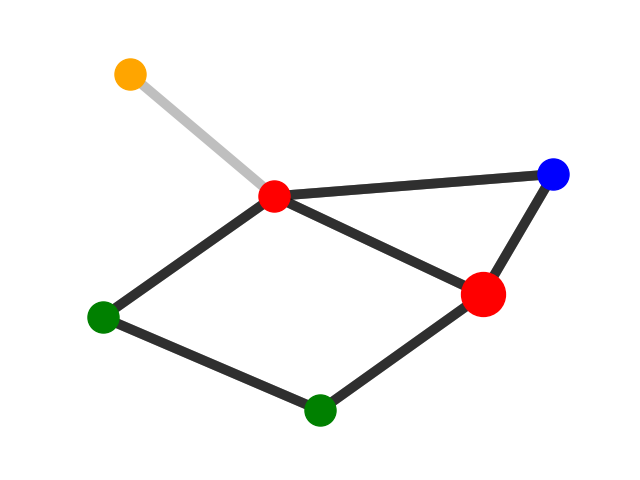
\includegraphics[width=.1\linewidth]{../openreview/imgs/extension/pg/syn1_good.png}
& 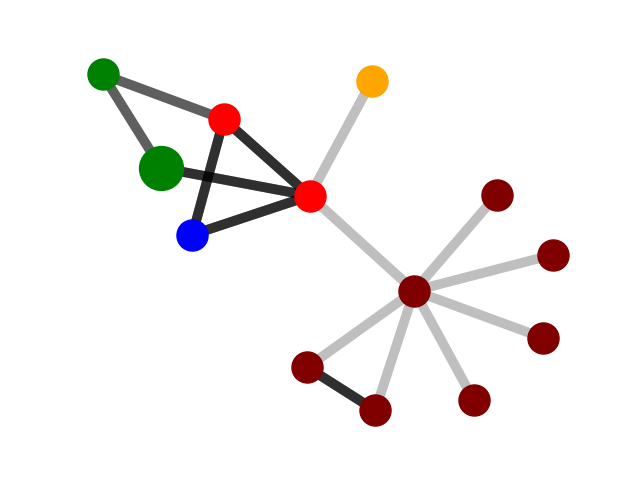
\includegraphics[width=.1\linewidth]{../openreview/imgs/extension/pg/syn2_good.png} & 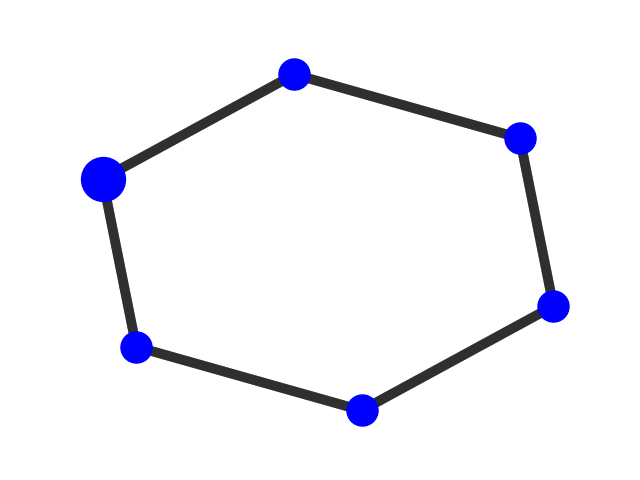
\includegraphics[width=.1\linewidth]{../openreview/imgs/extension/pg/syn3_good.png} & \multicolumn{1}{l|}{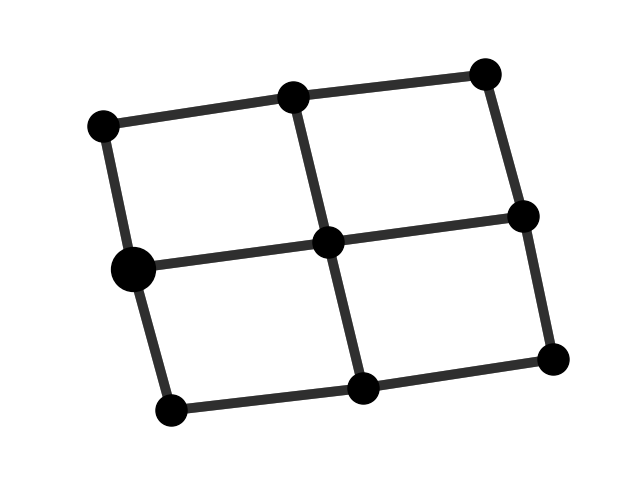
\includegraphics[width=.1\linewidth]{../openreview/imgs/extension/pg/syn4_good.png}} & \includegraphics[width=.1\linewidth]{../openreview/imgs/-5.png} & 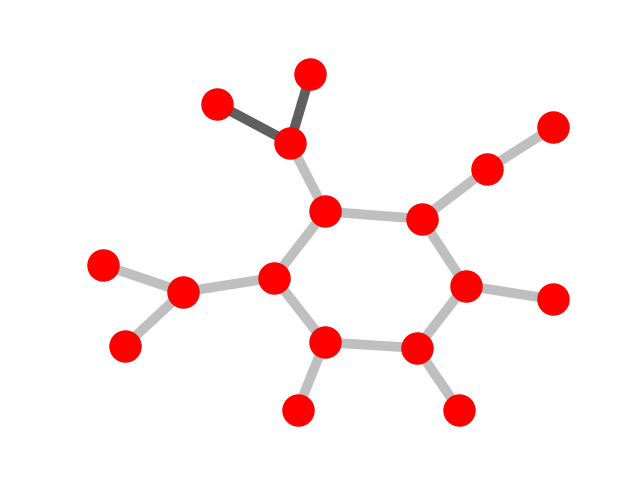
\includegraphics[width=.1\linewidth]{../openreview/imgs/extension/gnn/mutag_good.png} \\
PGExplainer (bad) &  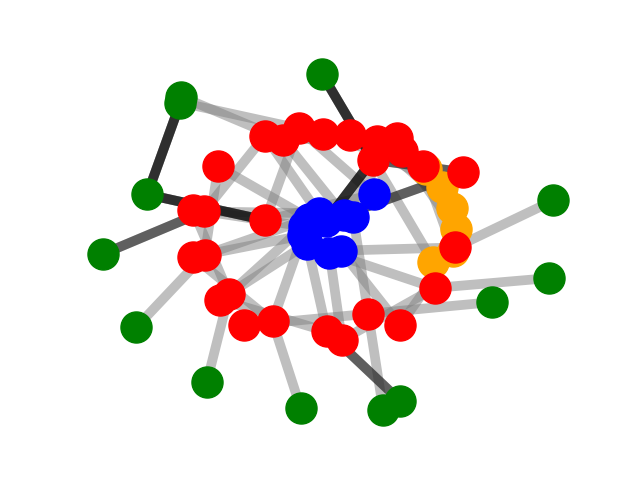
\includegraphics[width=.1\linewidth]{../openreview/imgs/extension/pg/syn1_bad.png}
& 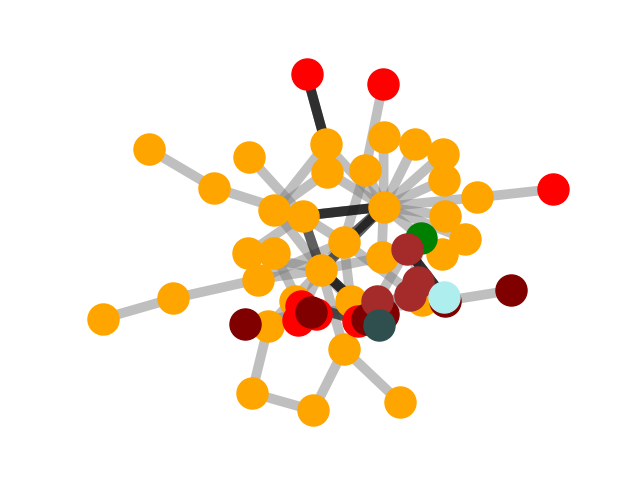
\includegraphics[width=.1\linewidth]{imgs/extension/pg/syn2_bad.png} & 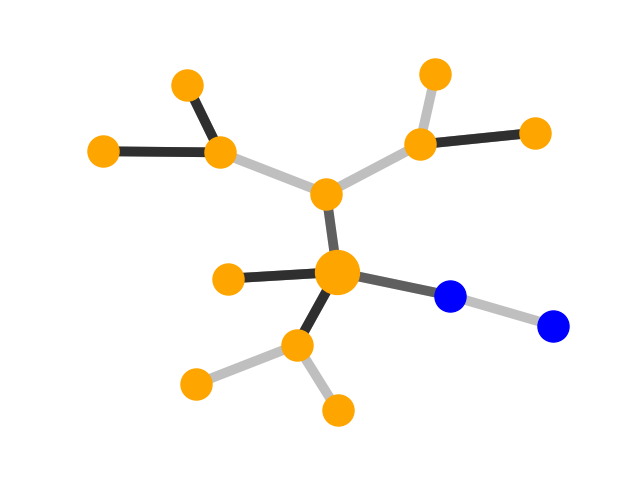
\includegraphics[width=.1\linewidth]{../openreview/imgs/extension/pg/syn3_bad.png} & \multicolumn{1}{l|}{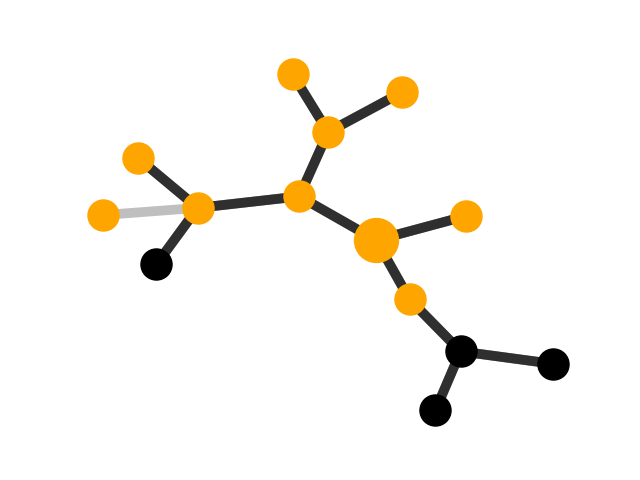
\includegraphics[width=.1\linewidth]{../openreview/imgs/extension/pg/syn4_bad.png}} & \includegraphics[width=.1\linewidth]{../openreview/imgs/-5.png} & 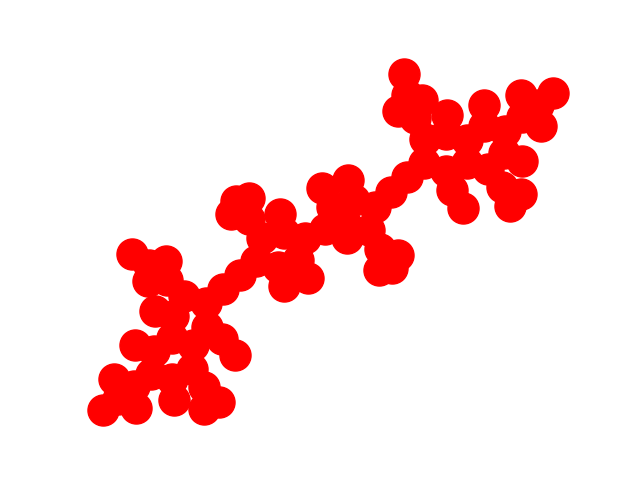
\includegraphics[width=.1\linewidth]{../openreview/imgs/extension/gnn/mutag_bad.png} \\
GNNExplainer (good) &  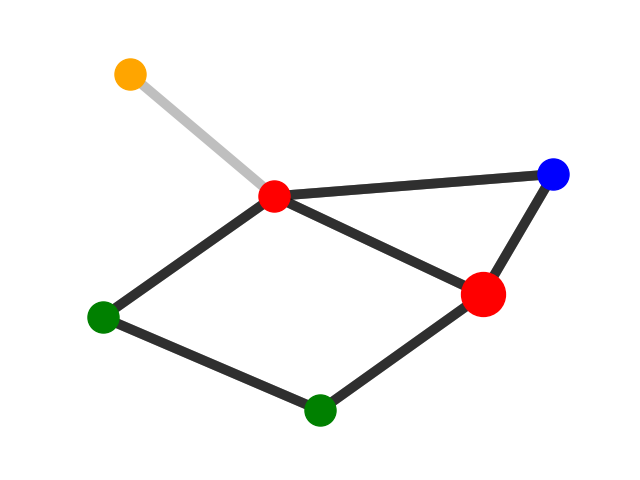
\includegraphics[width=.1\linewidth]{../openreview/imgs/extension/pg/syn1_good.png}
& 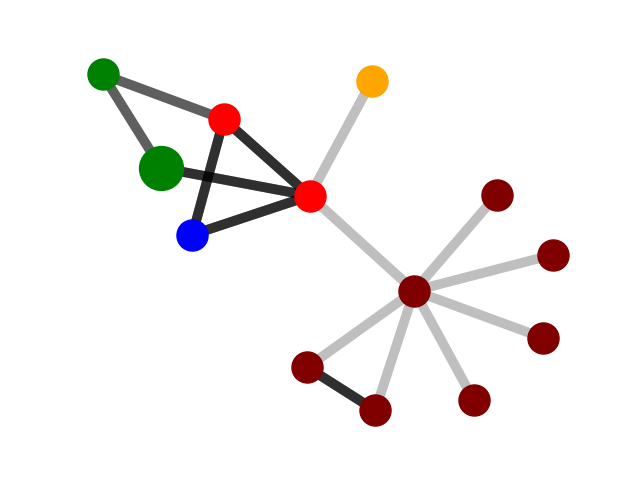
\includegraphics[width=.1\linewidth]{../openreview/imgs/extension/pg/syn2_good.png} & 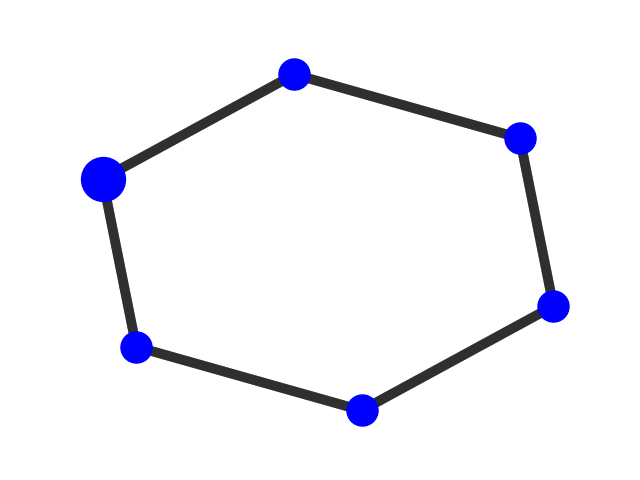
\includegraphics[width=.1\linewidth]{../openreview/imgs/extension/pg/syn3_good.png} & \multicolumn{1}{l|}{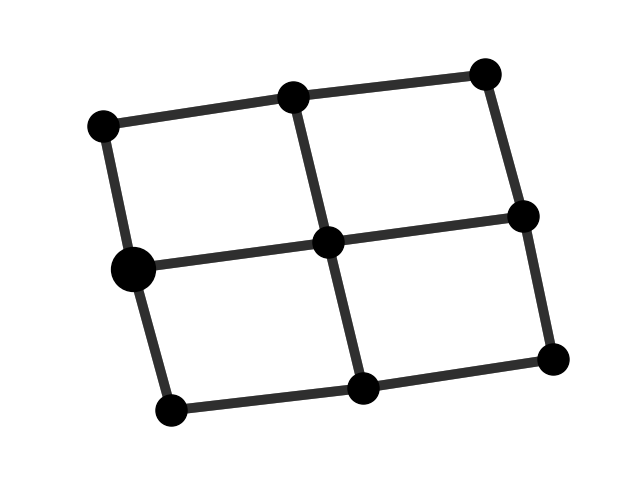
\includegraphics[width=.1\linewidth]{../openreview/imgs/extension/pg/syn4_good.png}} & \includegraphics[width=.1\linewidth]{../openreview/imgs/-5.png} & \includegraphics[width=.1\linewidth]{../openreview/imgs-6.png} \\
GNNExplainer (bad) &  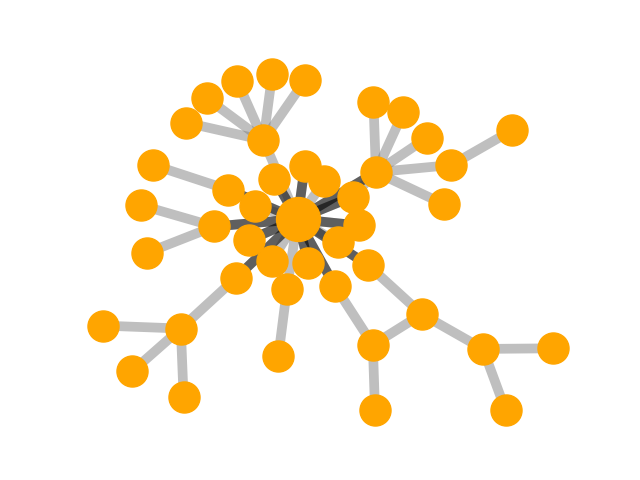
\includegraphics[width=.1\linewidth]{../openreview/imgs/extension/gnn/syn1_bad.png}
& 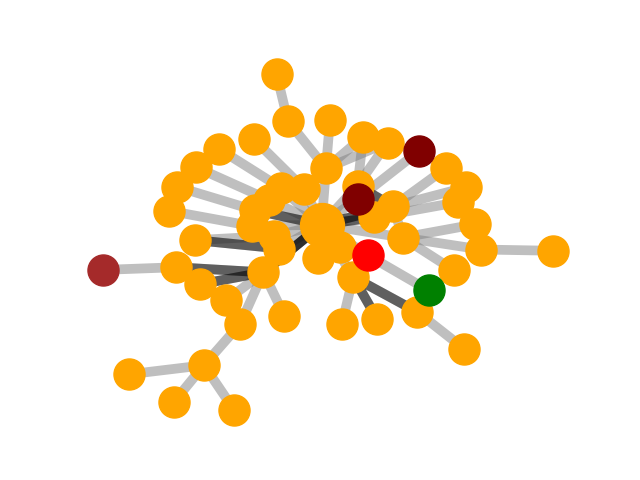
\includegraphics[width=.1\linewidth]{../openreview/imgs/extension/gnn/syn2_bad.png} & 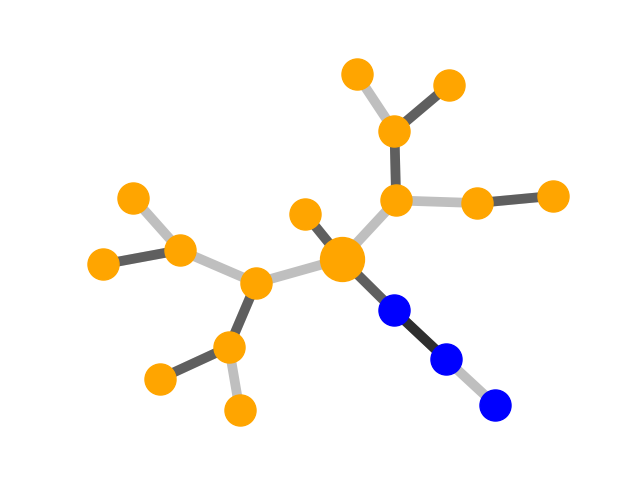
\includegraphics[width=.1\linewidth]{../openreview/imgs/extension/gnn/syn3_bad.png} & \multicolumn{1}{l|}{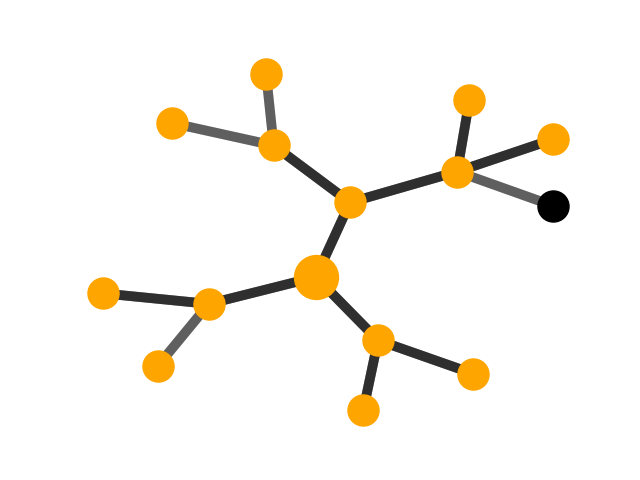
\includegraphics[width=.1\linewidth]{../openreview/imgs/extension/gnn/syn4_bad.png}} & \includegraphics[width=.1\linewidth]{../openreview/imgs/-5.png} & \includegraphics[width=.1\linewidth]{../openreview/imgs/-6.png} \\\hline
\multicolumn{7}{l}{\textbf{Explanation AUC}} \\ \hline
PGExplainer & 0.974 ± 0.005 & 0.576 ± 0.024 & 0.748 ± 0.014 & \multicolumn{1}{l|}{0.790 ± 0.009} & x.xx & 0.716 ± 0.166 \\ \hline
GNNExplainer & 0.508 ± 0.008 & 0.555 ± 0.002 & 0.482 ± 0.014 & \multicolumn{1}{l|}{0.608 ± 0.009} & x.xx & x.xx \\ \hline
\multicolumn{7}{l}{\textbf{Inference Time (ms)}} \\ \hline
PGExplainer & 17.96 & 46.1 & 17.6 & \multicolumn{1}{l|}{31.6} & x.xx & 32.32 \\
GNNExplainer & 54.30 & 78.25 & 25.81 & \multicolumn{1}{l|}{25.89} & x.xx & x.xx \\\bottomrule
\end{tabular}
\caption{Reproduction results}
\label{tab:reproduction_results2}
\end{table}


\subsection{Discussion}
The results presented in the extended reproduction seem to be in line with the claims related to the GNNExplainer by the authors of the PGExplainer. Both in terms of accuracy and efficiency, the PGExplainer outperforms the GNNExplainer by a significant margin. However, the handling of ground-truth explanations remains inconsistent for the presented datasets. While the improvements in the evaluation pipeline, such as not using the training set for evaluation, might have improved the validity of the claims the usefulness of the used ground-truth explanations remain questionable. 